\section*{Introduction}
Les appels système dans un système Linux embarqué sont des interfaces permettant aux applications d'interagir avec le noyau du système d'exploitation. Ils sont essentiels pour effectuer des opérations nécessitant des privilèges élevés ou un accès direct au matériel, généralement non autorisé pour les programmes utilisateur.

\textbf{Gestion des fichiers :}
\begin{itemize}
    \item \texttt{open() :} Pour ouvrir un fichier.
    \item \texttt{read() :} Pour lire à partir d'un fichier.
    \item \texttt{write() :} Pour écrire dans un fichier.
    \item \texttt{close() :} Pour fermer un fichier ou un descripteur de fichier.
\end{itemize}

\textbf{Gestion des processus :}
\begin{itemize}
    \item \texttt{fork() :} Pour créer un nouveau processus.
    \item \texttt{exec() :} Pour exécuter un nouveau programme dans le contexte du processus actuel.
    \item \texttt{wait() :} Pour attendre la fin d'un processus fils.
\end{itemize}

\textbf{Gestion des ressources système :}
\begin{itemize}
    \item \texttt{malloc() et free() :} Pour allouer et libérer de la mémoire dynamique.
    \item \texttt{brk() :} Pour ajuster la limite du segment de données.
\end{itemize}

\textbf{Gestion des fichiers et répertoires :}
\begin{itemize}
    \item \texttt{mkdir() :} Pour créer un répertoire.
    \item \texttt{rmdir() :} Pour supprimer un répertoire.
\end{itemize}

\textbf{Gestion des droits d'accès :}
\begin{itemize}
    \item \texttt{chmod() :} Pour modifier les permissions d'un fichier.
    \item \texttt{chown() :} Pour modifier le propriétaire d'un fichier.
\end{itemize}
\section{	Mise à jour du système}
sudo apt update && sudo apt upgrade
\section{	Installation des outils de développement}
sudo apt install gcc build-essential libncurses-dev libssl-dev libelf-dev bison flex -y
 \begin{figure}[h]
    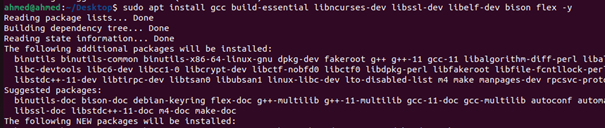
\includegraphics[width=1\textwidth]{images/25.png}   
\end{figure}
\section{Installation de l'outil "dwarves"}
sudo apt install dwarves
 \begin{figure}[h]
    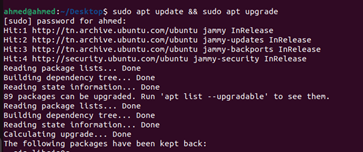
\includegraphics[width=1\textwidth]{images/26.png}   
\end{figure}
\section{	Nettoyage du système}
sudo apt clean && sudo apt autoremove -y
 \begin{figure}[h]
    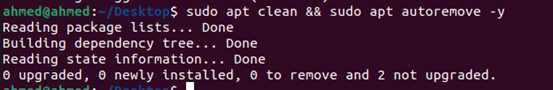
\includegraphics[width=1\textwidth]{images/27.png}   
\end{figure}
\section{	Téléchargement du noyau Linux 5.19.1}
wget -P ~/ https://mirrors.edge.kernel.org/pub/linux/kernel/v5.x/linux-5.19.1.tar.xz
 \begin{figure}[h]
    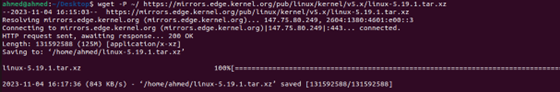
\includegraphics[width=1\textwidth]{images/28.png}   
\end{figure}
\section{Extraction des fichiers du noyau Linux 5.19.1}
tar -xvf ~/linux-5.19.1.tar.xz -C ~/
\section{Redémarrage système}
Rebbot
\section{Création d'un répertoire "helloworld" dans le répertoire "linux-5.19.1"}
cd linux-5.19.1
\\mkdir helloworld
\section{	Création du fichier "helloworld.c" dans le répertoire "helloworld"}
\begin{figure}[h]
    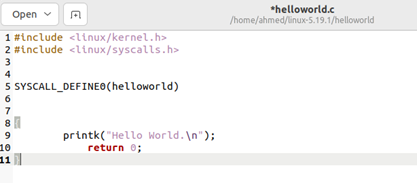
\includegraphics[width=1\textwidth]{images/29.png}   
\end{figure}
Le fichier \texttt{helloworld.c} contient un exemple de code pour créer un nouveau système d'appel (syscall) personnalisé dans le noyau Linux. Voici une explication détaillée de ce code :

\begin{itemize}
    \item Les fichiers d'en-tête \texttt{linux/kernel.h} et \texttt{linux/syscalls.h} sont inclus. Le premier contient des définitions et des structures utilisées par le noyau, tandis que le second contient des définitions et des structures spécifiques aux appels système.

    \item La fonction \texttt{SYSCALL\_DEFINE0(helloworld)} est définie. Cette macro est utilisée pour définir une nouvelle entrée de table de la table des appels système. La macro prend en argument le nom de la fonction et un ensemble d'arguments représentant les arguments passés à l'appel système.

    \item Le code suivant est simplement vide et est utilisé pour organiser le code.

    \item L'appel \texttt{printk("Hello World. \textbackslash n");} est utilisé pour afficher le message "Hello World." sur la console du système.

    \item Enfin, la fonction retourne 0, ce qui signifie que l'appel système s'est terminé avec succès.
\end{itemize}
\section{Création du fichire Makefile}
\begin{figure}[h]
    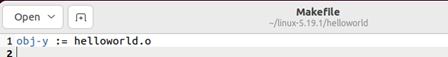
\includegraphics[width=1\textwidth]{images/30.png}   
\end{figure}
"obj-y := helloworld.o" dans un Makefile indique que le fichier objet "helloworld.o" doit être généré lors de la compilation du projet.

\section{Modification du fichier "Makefile}
\begin{figure}[h]
    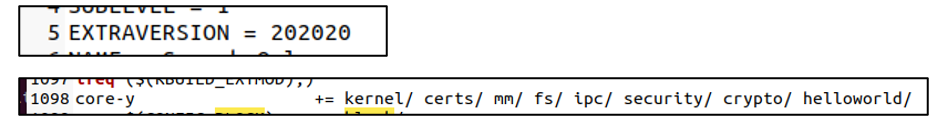
\includegraphics[width=1\textwidth]{images/31.png}   
\end{figure}
La modification du fichier "Makefile" en ajustant la variable d'extraversion et en ajoutant "helloworld" à la liste "core-y" après "block/" permet d'inclure le module "helloworld" dans la compilation du noyau Linux, tout en spécifiant la version du noyau cible, facilitant ainsi la personnalisation du noyau pour une configuration spécifique.
\section{Modification du fichier "syscalls.h" }
\begin{figure}[h]
    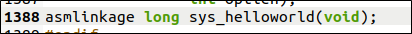
\includegraphics[width=1\textwidth]{images/32.png}   
\end{figure}
La modification du fichier "syscalls.h" pour ajouter une nouvelle déclaration de fonction système "sys\_helloworld" permet d'exposer une nouvelle fonction système dans le noyau Linux, que les programmes utilisateur peuvent appeler, étendant ainsi les fonctionnalités du noyau.
\section{Modification du fichier "syscall\_64.tbl}
\begin{figure}[h]
    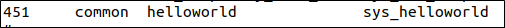
\includegraphics[width=1\textwidth]{images/33.png}   
\end{figure}
La modification du fichier "syscall\_64.tbl" pour ajouter l'entrée de la fonction système "sys\_helloworld" permet d'associer un numéro de syscall unique à cette nouvelle fonction système, permettant ainsi aux programmes utilisateur d'appeler la fonction "sys\_helloworld" de manière systématique en utilisant ce numéro de syscall spécifique. Cela garantit une interface cohérente pour accéder aux fonctionnalités ajoutées au noyau.
\newpage
\section{Configuration du noyau Linux en utilisant le menu de configuration}
sudo make menuconfig
\begin{figure}[h]
    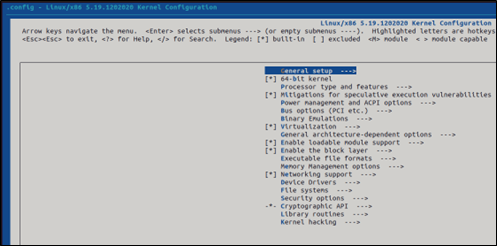
\includegraphics[width=1\textwidth]{images/34.png}   
\end{figure}
\section{Modification du fichier .conf}
\begin{figure}[h]
    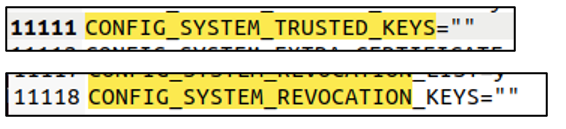
\includegraphics[width=1\textwidth]{images/35.png}   
\end{figure}
La modification du fichier de configuration du noyau Linux ("config") en supprimant le contenu entre les guillemets pour les options "CONFIG\_SYSTEM\_TRUSTED\_KEYS" et "CONFIG\_SYSTEM\_REVOCATIONS\_KEYS" signifie que l'on désactive la gestion des clés de confiance et des révocations du système, renforçant ainsi la sécurité du noyau en éliminant ces fonctionnalités potentiellement vulnérables.
\begin{figure}[h]
    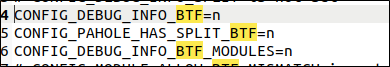
\includegraphics[width=1\textwidth]{images/36.png}   
\end{figure}
En changeant ces options de "y" à "n" dans la configuration du noyau Linux, vous désactivez la génération et l'utilisation de fichiers de débogage BTF (BPF Type Format). Cela réduit la taille de l'image du noyau et peut améliorer les performances, mais cela signifie que certaines fonctionnalités de débogage BTF ne seront pas disponibles, ce qui peut rendre le débogage plus difficile. Cette modification est généralement effectuée pour optimiser la configuration du noyau pour des scénarios spécifiques, comme les systèmes embarqués où l'espace disque est limité.
\section{Affichage du nombre de processeurs}
\begin{figure}[h]
    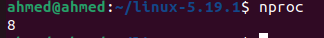
\includegraphics[width=0.7\textwidth]{images/37.png}   
\end{figure}
\section{Compilation du noyau}
\textbf{sudo make -j8}

\\La commande "make" est utilisée pour compiler et construire le noyau Linux, ainsi que d'autres composants du système. L'option "-j8" indique le nombre de tâches parallèles à exécuter lors de la compilation (8 dans cet exemple). En résumé, "make" est essentiel pour générer les binaires et les fichiers système nécessaires au fonctionnement du système embarqué Linux.
\section{18-	Installation des modules du noyau Linux }
\textbf{sudo make modules\_install -j8}
\begin{figure}[h]
    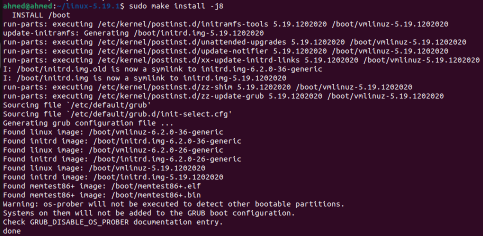
\includegraphics[width=1\textwidth]{images/39.png}   
\end{figure}

\section{Modification du fichier GRUB }
La configuration du fichier GRUB a été modifiée en passant du mode d'affichage automatique à un menu avec un délai de 10 secondes, permettant une sélection plus souple du noyau Linux au démarrage.
\newpage
\begin{figure}[h]
    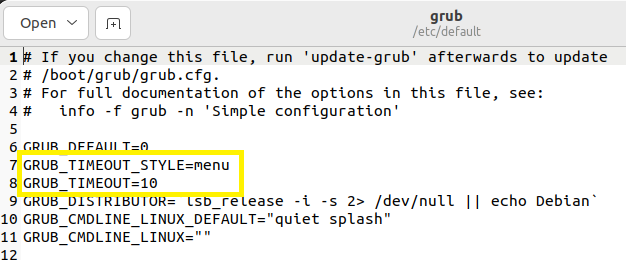
\includegraphics[width=0.8\textwidth]{images/40.png}   
\end{figure}
\section{Mise à jour du gestionnaire de démarrage GRUB }
\textbf{sudo update-grub}
\begin{figure}[h]
    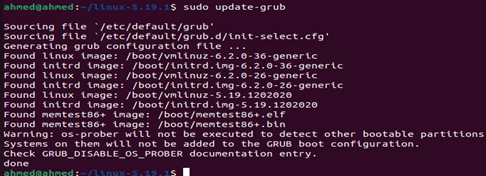
\includegraphics[width=0.8\textwidth]{images/41.png}   
\end{figure}

\section{Redémarrage du système pour démarrer avec le nouveau noyau Linux}
\begin{figure}[h]
    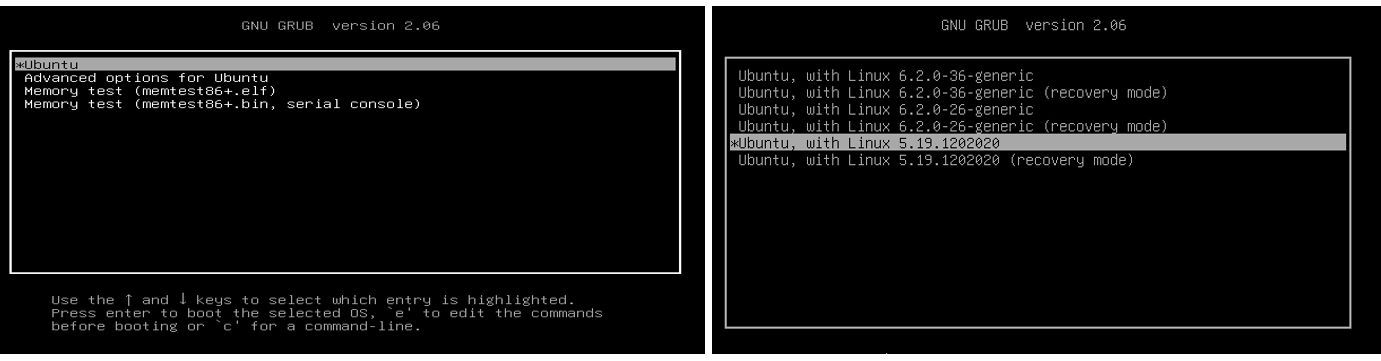
\includegraphics[width=0.8\textwidth]{images/42.png}   
\end{figure}

\section{Création du fichier testapellesystem }
\begin{figure}[h]
    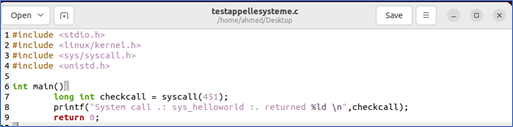
\includegraphics[width=0.8\textwidth]{images/43.png}   
\end{figure}
Ce programme est conçu pour appeler un appel système personnalisé (nommé "sys\_helloworld") et afficher le résultat de cet appel sur la sortie standard. La valeur renvoyée par l'appel système peut être utilisée pour communiquer des informations entre le noyau et l'application utilisateur.

\section{Compilation du programme C "testappellesysteme.c" }
\begin{figure}[h]
    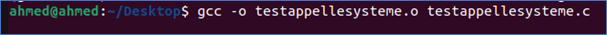
\includegraphics[width=0.8\textwidth]{images/44.png}   
\end{figure}
\section{Exécution du programme "testappellesysteme.o" }
\begin{figure}[h]
    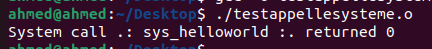
\includegraphics[width=0.8\textwidth]{images/45.png}   
\end{figure}

\section{Exécution de la commande dmesg pour afficher les messages du noyau}
\begin{figure}[h]
    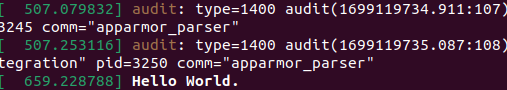
\includegraphics[width=0.8\textwidth]{images/46.png}   
\end{figure}

La commande dmesg est utilisée dans les systèmes d'exploitation de type Unix, y compris Linux, pour afficher les messages du noyau du système. Le nom "dmesg" signifie "display message" (afficher les messages). Cette commande permet d'examiner les messages générés par le noyau Linux pendant le processus de démarrage du système et fournit des informations sur les événements du noyau, les erreurs, les avertissements et d'autres activités liées au matériel.

\section*{Conclusion}
Cette tache a s’agit  d’un processus complet de création d'un module de noyau Linux nommé "helloworld". Les étapes comprenaient l'installation d'outils, le téléchargement d'une version du noyau Linux, la configuration du noyau pour ajouter un nouveau module, la modification de fichiers sources, la compilation du noyau, et l'exécution d'un programme utilisateur qui appelait la nouvelle fonction système. En fin de compte, ce projet  permet de mieux comprendre les bases de la création de modules de noyau, de la configuration du noyau, de l'appel de fonctions système depuis des programmes utilisateur, de la compilation et de l'installation d'un noyau personnalisé.
